\documentclass[fr,license=none]{../../../eplexercises}
\usepackage{multido}
\usepackage{float}
\usepackage{../../../eplcode}
\usepackage{../../../eplunits}
\usepackage{siunitx}
\usepackage{listings}
\usepackage{amsmath}

% General info
\hypertitle[e ]{Systèmes informatiques 1}{3}{SINF}{1252}
{Brieuc Kaisin \and Cynthia Laureys \and Jean-Martin Vlaeminck}
{Olivier Bonaventure}
 
 
 % New colors
\definecolor{codegreen}{rgb}{0,0.6,0}
\definecolor{codegray}{rgb}{0.5,0.5,0.5}
\definecolor{backcolour}{rgb}{0.95,0.95,0.92}

\lstdefinestyle{mystyle}{
    backgroundcolor=\color{backcolour},   
    commentstyle=\color{codegreen},
    keywordstyle=\color{RedViolet},
    numberstyle=\tiny\color{codegray},
    stringstyle=\color{red},
    %basicstyle=\footnotesize,
    basicstyle=% change it if you want
        \ttfamily%
        \normalsize,
        %\lst@ifdisplaystyle\normalsize\fi,
    breakatwhitespace=false,         
    breaklines=true,                 
    captionpos=b,                    
    keepspaces=true,                 
    numbers=left,                    
    numbersep=5pt,                  
    showspaces=false,                
    showstringspaces=false,
    showtabs=false,                  
    tabsize=2,
    literate=%
    {é}{{\'e}}1
    {è}{{\`e}}1
    {à}{{\`a}}1
}


\lstset{style=mystyle, language=C}

%----------------------------------Macros--------------------------------------

\titleformat
{\section} % command
[display] % shape
{\bfseries\Large} % format
{\newpage Semaine \thesection} % label
{0.5ex} % sep
{} % before-code


\titleformat
{\subsection} % command
{\normalfont\large\bfseries} % format
{\thesubsection} % label
{0.5ex} % sep
{} % before-code

\newcommand\TODO{\textcolor{red}{TO DO}}
\newcommand\question[1]{\medskip\noindent\underline{\textbf{Question #1 :}}}
\newcommand\ingi[2]{\begin{center}\textbf{#1}\\ \url{#2}\end{center}}

\newcommand\qcm[2]
{
	\multido{\i=1+1}{#2}{
    \begin{figure}[H]
    	\centering
        \includegraphics[width=14cm]{#1/Q\i.PNG}
    \end{figure}}
}
%------------------------------------------------------------------------------   




%--------------------------------------S1--------------------------------------
\section{Introduction à Unix et au langage C} %1
\pagenumbering{arabic}
\subsection{QCM}
\qcm{QCMS1}{5}

\subsection{Exercices en bash}
\TODO

\subsection{Questions de base}
\question{1,2,6}
\begin{description}
\item[-Werror] Make all warnings into errors.
\item[-Wall] This enables all the warnings about constructions that some
users consider questionable, and that are easy to avoid (or modify to
prevent the warning), even in conjunction with macros. This also enables
some language-specific warnings described in C++ Dialect Options and
Objective-C and Objective-C++ Dialect Options.
\item[(-Wfatal-errors] This option causes the compiler to abort compilation
on
the first error occurred rather than trying to keep going and printing further
error messages.)
\end{description}

\question{3,7} Il faut rajouter \textit{return 0;} par exemple.

\question{8}
\url{http://sites.uclouvain.be/SystInfo/manpages/man3/atoi.3.html}\\
\url{http://sites.uclouvain.be/SystInfo/manpages/man3/strtol.3.html}

\question{9} EASY

\question{10} \TODO

\subsection{Petits programmes}

\question{1} \url{http://sites.uclouvain.be/SystInfo/manpages/man1/test.1.html}
\ingi{La commande test}{https://inginious.info.ucl.ac.be/course/LSINF1252/commandetest}
\begin{lstlisting}
#include <stdlib.h>
#include <stdio.h>
#include <string.h>

int eq(int n1, int n2)
{
	if(n1 == n2)
	return 0;
	else
	return 1;
}
int ge(int n1, int n2)
{
	if(n1 >= n2)
	return 0;
	else
	return 1;
}
int gt(int n1, int n2)
{
	if(n1 > n2)
	return 0;
	else
	return 1;
}
int le(int n1, int n2)
{
	if(n1 <= n2)
	return 0;
	else
	return 1;
}
int lt(int n1, int n2)
{
	if(n1 < n2)
	return 0;
	else
	return 1;
}
int ne(int n1, int n2)
{
	if(n1 != n2)
	return 0;
	else
	return 1;
}

int main(int argc, char *argv[])
{
	if(argc == 4)
	{
		int n1 = atoi(argv[1]);
		int n2 = atoi(argv[3]);
		
		if(strcmp(argv[2],"-eq") == 0)
			return eq(n1,n2);
		else if(strcmp(argv[2],"-ge") == 0)
			return ge(n1,n2);
		else if(strcmp(argv[2],"-gt") == 0)
			return gt(n1,n2);
		else if(strcmp(argv[2],"-le") == 0)
			return le(n1,n2);
		else if(strcmp(argv[2],"-lt") == 0)
			return lt(n1,n2);
		else if(strcmp(argv[2],"-ne") == 0)
			return ne(n1,n2);
		else
		printf("bad instruction ");
	}
	else
	{
		printf("Incorrect number of arguments (%d argument(s))\n",argc);
	}
	return 1;
}
\end{lstlisting}

\question{2} Fort semblable à la question 1.\\
\url{http://sites.uclouvain.be/SystInfo/manpages/man1/expr.1.html}

\question{3} \TODO

%--------------------------------------S2--------------------------------------
\section{Types de données} %2
\subsection{QCM}
\qcm{QCMS2}{13}

\subsection{Questions de base}
\question{1}
\begin{lstlisting}
#include <stdio.h>
#include <stdint.h>

int main(int argc, const char *argv[])
{
    printf("int : %d bytes\n", sizeof(int));
    printf("long : %d bytes\n", sizeof(long));
    printf("void* : %d bytes\n", sizeof(void *));
    printf("char* : %d bytes\n", sizeof(char *));
    printf("size_t : %d bytes\n", sizeof(size_t));
    printf("uint64_t : %d bytes\n", sizeof(uint64_t));
}
\end{lstlisting}

\question{2}
\begin{lstlisting}
void lsb(int number)
{
    int nbr = number;
    int bit = 32;
    while (nbr!=0)
    {
        nbr<<=1;
        bit--;
        //amelioration : effectuer bit-- avec des operations binaires
    }
    printf("Less significant bit of %d : %d", number, (int) pow(2,bit));
}
\end{lstlisting}

\question{3}
\begin{lstlisting}
#include <stdio.h>

int main()
{
    char* ptr = "Test";
    int i;
    for (i=0 ; i<4 ; i++){
        printf("%p\n", (void *) (ptr+i)); //or &ptr[i]
    }
}
\end{lstlisting}

\question{4}
\ingi{Echange de valeurs de fractions}{https://inginious.info.ucl.ac.be/course/LSINF1252/swap}
\begin{lstlisting}
void swap(struct fract_t *a, struct fract_t *b)
{
    int mem1 = a->num;
    int mem2 = a->denum;
    a->num = b->num;
    a->denum = b->denum;
    b->num = mem1;
    b->denum = mem2;
}
\end{lstlisting}

\question{5}
\begin{lstlisting}
#include <stdio.h>

int main()
{
    struct foo_t
    {
        char a;
        int b;
    };
    printf("Size of struct foo_t : %d bytes",sizeof(struct foo_t));
}
\end{lstlisting}

L'exécution de ce code affiche : \lstinline{Size of struct foo\_t : 8 bytes} et non 5 bytes (1+4) comme on pourrait le penser. Cela est dû à un phénomène d'alignement sur 32 bits du \textit{char a}.

\question{6}
\url{http://sites.uclouvain.be/SystInfo/manpages/man3/string.3.html}\\
\url{http://sites.uclouvain.be/SystInfo/manpages/man3/strlen.3.html}\\
\url{http://sites.uclouvain.be/SystInfo/manpages/man3/strcat.3.html}\\
\url{http://sites.uclouvain.be/SystInfo/manpages/man3/strcasecmp.3.html}\\
\textcolor{red}{Avertissement : ce code n'a pas encore été testé sur inginious (nombre d'essais limité)}

\ingi{Mini-projet : implémentation de strlen, strcat et strcasecmp}{https://inginious.info.ucl.ac.be/course/LSINF1252/mini-projet-string}
\begin{lstlisting}
size_t strlen(const char *str) {
    int i;
    for(i=0 ; str[i]!='\0';i++);
    return (size_t) i;
}

char *strcatt(char *destination, const char *source) {
    int i;
    int lenD = strlen(destination);
    int lenS = strlen(source);
    for (i=lenD ; i<lenD+lenS ; i++)
    {
        destination[i] = source[i-lenD];
    }
    destination[i+1] = '\0';
    return destination;
}

int strcasecmp(const char *s1, const char *s2) {
//TO DO
}
\end{lstlisting}

%--------------------------------------S3--------------------------------------
\section{Organisation de la mémoire} %3
\subsection{QCM}
\qcm{QCMS3}{7}

\subsection{Questions}

\question{1}
\begin{description}
\item[void *calloc(size\_t nmemb, size\_t size);] allocates memory for an array of
\textit{nmemb} elements of size bytes each and returns a pointer to the allocated
memory. The memory is set to zero. If \textit{nmemb} or size is 0, then
\textit{calloc()} returns either NULL, or a unique pointer value that can later be
successfully passed to \textit{free()}.
\item[void *malloc(size\_t size);] allocates \textit{size} bytes and returns a pointer
to the allocated memory. The memory is not cleared. If size is 0, then
\textit{malloc()} returns either NULL, or a unique pointer value that can later be
successfully passed to \textit{free()}.
\item[void free(void *ptr);] frees the memory space pointed to by \textit{ptr}, which
must have been returned by a previous call to \textit{malloc()}, \textit{calloc()} or
\textit{realloc()}. Otherwise, or if \textit{free(ptr)} has already been called
before, undefined behavior occurs. If ptr is NULL, no operation is performed.
\item[void *realloc(void *ptr, size\_t size);] changes the size of the memory block
pointed to by \textit{ptr} to \textit{size} bytes. The contents will be unchanged to
the minimum of the old and new sizes; newly allocated memory will be uninitialized. If
\textit{ptr} is NULL, then the call is equivalent to \textit{malloc(size)}, for all
values of \textit{size}; if \textit{size} is equal to zero, and \textit{ptr} is not
NULL, then the call is equivalent to \textit{free(ptr)}. Unless \textit{ptr} is NULL,
it must have been returned by an earlier call to \textit{malloc()}, \textit{calloc()}
or \textit{realloc()}. If the area pointed to was moved, a \textit{free(ptr)} is done.
\end{description}
\textit{calloc()} est plus lent que \textit{malloc()}.

\question{2} \TODO
\begin{lstlisting}
/**************************************
 * stack.c
 *
 * Programme d'exemple implementant un stack comme structure
 * chainee
 *
 **************************************/

#include <stdio.h>
#include <stdlib.h>

typedef struct fraction_t {
  int num;
  int den;
} fraction;

///AAA
typedef struct node_t
{
  struct fraction_t *data;
  struct node_t *next;
} node;

struct node_t *stack; // sommet de la pile

// ajoute un element au sommet de la pile
void push(struct fraction_t *f)
{
  struct node_t *n;
  n=(struct node_t *)malloc(sizeof(struct node_t));
  if(n==NULL)
    exit(EXIT_FAILURE);
  n->data = f;
  n->next = stack;
  stack = n;
}
// retire l'element au sommet de la pile
struct fraction_t * pop()
{
  if(stack==NULL)
    return NULL;
  // else
  struct fraction_t *r;
  struct node_t *removed=stack;
  r=stack->data;
  stack=stack->next;
  free(removed);
  return (r);
}

///BBB

// affiche le contenu de la pile
void display()
{
  struct node_t *t;
  t = stack;
  while(t!=NULL) {
    if(t->data!=NULL) {
      printf("Item at addr %p  :  Fraction %d/%d   Next %p\n",t,t->data->num,t->data->den,t->next);
    }
    else {
      printf("Bas du stack %p\n",t);
    }
    t=t->next;
  }
}

// exemple
int main(int argc, char *argv[]) {

  struct fraction_t demi={1,2};
  struct fraction_t tiers={1,3};
  struct fraction_t quart={1,4};
  struct fraction_t zero={0,1};

  // initialisation
  stack = (struct node_t *)malloc(sizeof(struct node_t));
  stack->next=NULL;
  stack->data=NULL;

  display();
  push(&zero);
  display(); %splay()
  push(&demi);
  push(&tiers);
  push(&quart);
  display();

  struct fraction_t *f=pop();
  if(f!=NULL)
    printf("Popped : %d/%d\n",f->num,f->den);

  return(EXIT_SUCCESS);
}
///CCC
\end{lstlisting}

\question{3}
\TODO

\question{4}
\TODO

\question{5}
\begin{lstlisting}
int main()
{
    int i;
    int a[3][3] = { {1,2,3} , {4,5,6} , {7,8,9} };
    int *b = &a;
    for(i=0 ; i<9 ; i++) printf("%d\n",*b+i);
    return 0;
}
\end{lstlisting}
Le programme affiche \textit{1,2,3,4,5,6,7,8,9}. Conclusion : le tableau \textit{a} est stocké ligne par ligne.

\question{6}
\begin{lstlisting}
int main()
{
    typedef struct
    {
        char c;
        long l;
        short s;
    } test_t;
    printf("Size of struct test_t : %d bytes",sizeof(test_t));
    return 0;
}
\end{lstlisting}
Le programme indique que la taille de la structure vaut 12 bytes.

\begin{lstlisting}
int main()
{
    typedef struct
    {
        char c;
        long l;
        short s;
    } test_t;
    test_t stru;
    stru.c = 4;
    stru.l = 456;
    stru.s = 42;
    int* ptrC = &stru.c;
    int* ptrL = &stru.l;
    int* ptrS = &stru.s;
    printf("%p, %p, %p",ptrC,ptrL,ptrS);
    return 0;
}
\end{lstlisting}
Le code ci-dessus affiche ceci : 0028FF14, 0028FF18, 0028FF1C.\\
Un moyen de réduire cette taille est d'écrire la structure ainsi :
\begin{lstlisting}
typedef struct
{
    char c;
    short s;
    long l;
} test_t;
\end{lstlisting}
Elle n'occupe maintenant plus que 8 bytes en mémoire.

\question{7}
\url{http://sites.uclouvain.be/SystInfo/manpages/man1/gcc.1.html}\\
\url{http://stackoverflow.com/questions/4306186/structure-padding-and-packing}
\begin{figure}[H]
\centering
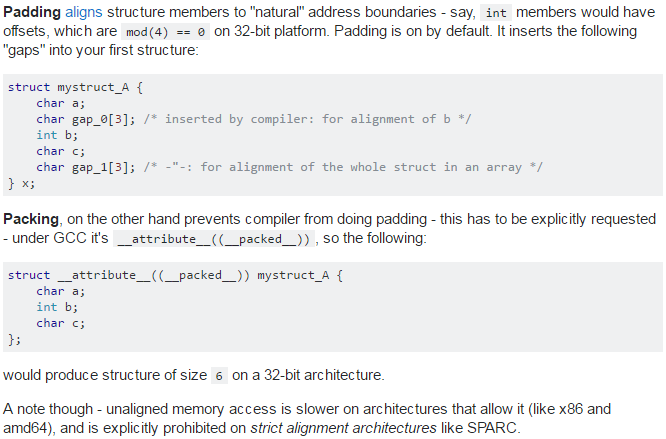
\includegraphics[width=14cm]{packed.PNG}
\end{figure}

\question{8}
\begin{lstlisting}
int global;
void main(void)
{
        int local;
        int *ptr1 = (int *)malloc(sizeof(*ptr1));
        int *ptr2 = (int *)malloc(sizeof(*ptr2));

        printf("global %p loc %p p1 %p p2 %p\n", &global, &local, ptr1, ptr2);
}
\end{lstlisting}
\TODO

\question{9}
\TODO

\question{10}
\ingi{Listes chaînées: concepts de base}{https://inginious.info.ucl.ac.be/course/LSINF1252/linked_lists_1}
\begin{lstlisting}
typedef struct node {
  int value;
  struct node *next;
} node;

size_t length(node *list)
{
    if(list==NULL)
        return 0;

    int count = 1;
    while (list->next != NULL)
    {
        list = list->next;
        count++;
    }

    return count;
}

size_t count(node *list, int value)
{
    if(list == NULL)
        return 0;

    int count = 0;
    while (list !=NULL)
    {
        if(list->value == value) count++;
        list = list->next;
    }
    return count;
}

int push(node **list, int value)
{
    node *n;
    n = (node *)malloc(sizeof(node));
    if(n == NULL)
        return -1;
    n->value = value;
    n->next = *list;
    *list = n;
    return 0;
}

int pop(node **list)
{
    if(list==NULL)
        return 0;

    int r;
    struct node *removed=*list;
    r = (*list)->value;
    *list = (*list)->next;
    free(removed);
    return r;
}

void free_list(node *list)
{
    struct node* tmp;

    while (list != NULL)
    {
        tmp = list;
        list = list->next;
        free(tmp);
    }
}
\end{lstlisting}

%--------------------------------------S4--------------------------------------
\section{Organisation des ordinateurs et étude de cas : IA32} %4
\subsection{QCM}
\TODO
\subsection{Exercices}

%--------------------------------------S5--------------------------------------
\section{Compléments de C et utilisation de plusieurs threads} %5
\subsection{QCM}
\TODO
\subsection{Exercices}

\question{1}
La fonction \lstinline|phtread_join| utilise un deuxième argument de type \lstinline|void**|. Pourquoi est-il nécessaire d'utiliser un pointeur vers un pointeur et pas simplement un \lstinline|void*| ?

\begin{solution}
Souvent, nos threads vont vouloir retourner un pointeur vers une zone mémoire allouée
sur le tas. C'est pour ça que nos threads retournent \lstinline{void*}.

Du coup, \lstinline{pthread_join} doit recevoir un pointeur vers une variable du même
type que ce qu'on retourne, vu qu'elle va modifier la variable. Ce qu'on retourne
étant un \lstinline{void*}, l'argument de \lstinline{pthread_join} doit être un \lstinline{void**}.
\begin{itemize}
    \item \lstinline{void} ou tout autre type ne servirait à rien : \lstinline{pthread_join} ne
    pourrait pas modifier la moindre variable pour l'utilisateur.
    \item \lstinline{void*} ne permet que de retourner une valeur non-pointeur, et pas un pointeur
    (sauf en faisant un cast, ce qui est très dégueulasse). \lstinline{pthread_join} peut par
    exemple mettre un \lstinline{int}, mais pas un \lstinline{int*}
    \item \lstinline{void**} permet à \lstinline{pthread_join} de modifier l'argument et d'éventuellement y
    mettre un pointeur générique (\lstinline{void*})
\end{itemize}
\end{solution}

\question{2}
À votre avis, pourquoi le premier argument de la fonction \lstinline|pthread_create| est-il un pointeur de type \lstinline|pthread_t*| alors que le premier argument de la fonction \lstinline|pthread_joind| est lui simplement de type \lstinline|pthread_t| ?

\begin{solution}
\lstinline{pthread_create} doit modifier la structure qu'on lui passe en argument (il doit l'initialiser), tandis que \lstinline{pthread_join} se contente d'accéder aux valeurs qu'on lui passe en argument, et ne les modifie pas.
\end{solution}

\question{3}
Avec les threads POSIX, comment peut-on passer plusieurs arguments à la fonction démarrée par \lstinline|pthread_create| ? Écrivez un petit exemple en C qui permet de passer un entier et un caractère à cette fonction.

\begin{solution}
La manière la plus simple de le faire est de définir une structure contenant un entier et un caractère, et de passer un pointeur vers cette structure au thread. Par exemple,

\lstinputlisting[linerange={7-33}]{src/ape5q3.c}
\end{solution}

\question{4}
Ecrivez un code qui permet de récupérer un tableau d’entiers d’un thread. Exercice disponible sur \href{https://inginious.info.ucl.ac.be/course/LSINF1252/threads_1}{INGInious}.

\begin{solution}
Faites l'exercice par vous-même ;-).

De manière générale, lorsqu'un thread doit renvoyer une structure de données complexe, ou plusieurs valeurs de retour (tableau statique dont la taille n'est pas connue, liste chainée, tableau et sa taille, plusieurs valeurs de retour), une manière propre de renvoyer ces résultats est de renvoyer une structure spécialement conçue pour retourner toutes ces valeurs. Par exemple, s'il faut renvoyer une liste chainée de mots de passe définie par une \lstinline|struct PasswordList|, ainsi qu'un entier indiquant le nombre total de mots de passe traités (mais pas nécessairement compris dans la liste), on pourrait déclarer une structure
\begin{lstlisting}
struct ThreadReturn {
	int nbrProcessedPasswords;
	struct PasswordList *list;
};
\end{lstlisting}
et le thread retournerait alors un pointeur sur une telle structure : la signature resterait \lstinline|void *my_thread(void *param)| mais les dernières lignes de la fonction seraient
\begin{lstlisting}
struct ThreadReturn *ret = (struct ThreadReturn*) malloc(sizeof(struct ThreadReturn));
if (ret == NULL)
	return NULL;
ret->list = liste; // la liste de mots de passe
ret->nbrProcessedPasswords = nbreMDP; // le nombre de mots de passe lus
return (void*) ret;
\end{lstlisting}
ce qui permet de retourner toutes les valeurs de retour.
\end{solution}

\question{5}
Essayez de lancer un grand nombre de threads d'exécution sur votre machine. Quel est le nombre maximum de threads que \lstinline|phtread_create| vous autorise à lancer ?

\begin{solution}
Environ $3000$ threads. En tout cas, c'est le maximum de ce qu'il est possible d'avoir sans qu'une segfault plutôt embêtante survient. On peut théoriquement en lancer $100000$ en réduisant la tâche qu'ils doivent accomplir, mais au bout d'un moment les threads lancés au début finissent par se terminer, libérant de la place pour les nouveaux.

Toutes ces valeurs dépendent de l'ordinateur sur lequel les programmes sont utilisés.
\end{solution}

\question{6}
Quelle différence voyez-vous entre \lstinline|pthread_exit| et \lstinline|exit| ?

\begin{solution}
\lstinline{pthread_exit} équivaut à un return dans une des fonctions de thread : ça arrête le thread courant.

\lstinline{exit} équivaut à un \lstinline{return} dans la fonction main : ça arrête le programme.
\end{solution}

\question{7}
Un étudiant souhaite passer un tableau d'entiers comme argument à un thread et écrit le code suivant : \href{https://github.com/obonaventure/SystemesInformatiques/blob/master/Exercices/Programmes/src/pthread-array.c}{/Programmes/src/pthread-array.c}. Qu'en pensez-vous ?

\begin{solution}
Lors de la fin de l'appel à \lstinline{launch} (qui s'exécute assez rapidement), le tableau \lstinline{v} alloué sur la pile n'est plus accessible, les threads qui s'exécutent reçoivent donc une valeur incorrecte et donc le programme foire (bon, c'est du garbage mais quand même).
\end{solution}

\question{8}
Considérons le programme de test des threads POSIX disponible à l'adresse \url{http://sites.uclouvain.be/SystInfo/notes/Exercices/html/_downloads/pthread-test.c}. Ce programme utilise 4 threads qui incrémentent chacun un million de fois une variable globale.
Exécutez ce programme et observez le résultat qu'il affiche à l'écran. Pouvez-vous expliquer le comportement de ce programme ?

\begin{solution}
De manière assez évidente, on n'atteint jamais $40000000$ mais des trucs intermédiaires : il est fort probable que deux threads exécutent \lstinline|global=increment(global)| en même temps, ce qui a pour conséquence de n'incrémenter \lstinline|global| qu'une fois. Il aurait fallu utiliser des mutex.
\end{solution}

\question{9}
Résolvez des sudokus. Exercice disponible sur INGInious : \url{https://inginious.info.ucl.ac.be/course/LSINF1252/sudoku}

\begin{solution}
Faites l'exercice par vous-même ;-), même s'il n'est pas très intéressant.
%Implémenter un solveur de sudoku en utilisant un algorithme de remplissage aléatoire. Pas très intéressant, mais TODO
\end{solution}


\subsection{Mini-projet : mesure de performance}



% //====================================================\\
% ||                         S6                         ||
% \\====================================================//

\section{Communication entre threads}
\subsection{QCM}
\TODO

\subsection{Exercices}

\question{1}
Écrivez un petit programme qui vous permet de montrer quelles variables sont accessibles à différents threads. Les variables à montrer sont:
\begin{itemize}
	\item variable globale statique
	\item variable globale
	\item variable déclarée dans la fonction main et dont le pointeur est un des arguments aux threads
	\item variable statique déclarée à l’intérieur d’une fonction
	\item variable locale déclarée dans une fonction
\end{itemize}

\begin{solution}
Les variables accessibles aux threads sont :
\begin{itemize}
    \item les variables globales;
    \item les variables dont un pointeur est l'argument d'un des threads;
    \item et les variables globales statiques si la fonction du thread est dans le même fichier (err, \emph{compilation unit}) que cette variable.
\end{itemize}

La variables statique à une fonction n'est accessible que de cette fonction, mais sa valeur est "commune" à chaque thread, ce qui fait que ladite fonction n'est \emph{a priori} pas thread-safe.

La variable locale est évidemment accessible qu'à partir de la fonction, et est réinitialisée à chaque appel de la fonction.
\end{solution}

\question{2}
D’après vous (essayez d’expérimenter), que se passe-t-il si:
\begin{itemize}
	\item un thread exécute deux fois \lstinline|pthread_mutex_lock| sur le même mutex d’affilée ?
	\item un thread exécute deux fois d’affilée \lstinline|pthread_mutex_unlock| ?
\end{itemize}

\begin{solution}
Plusieurs fois \lstinline|pthread_mutex_lock| : il se deadlock lui-même. Sauf si on a créé un mutex avec gestion des erreurs (\lstinline|PTHREAD_MUTEX_ERRORCHECK|) ; là il détecte le deadlock et renvoie une erreur.

Plusieurs fois \lstinline|pthread_mutex_unlock| : \emph{undefined behaviour} (en clair, ça crashe, ou alors ça délocke le mutex dans un autre thread, ce qui est rarement voulu).
\end{solution}

\question{3}
Dans la partie théorie, nous avons vu comment s’assurer qu’un seul thread peut accéder à une zone critique à la fois. On vous propose deux solutions (dont une déjà vue dans la partie théorie) :
\begin{lstlisting}
pthread_mutex_lock(&mutex_global);
global=increment(global);
pthread_mutex_unlock(&mutex_global);
\end{lstlisting}
et
\begin{lstlisting}
while (pthread_mutex_trylock(&mutex_global)) ;
global=increment(global);
pthread_mutex_unlock(&mutex_global);
\end{lstlisting}
Discuter les avantages et inconvénients des ces deux solutions (regardez la man page de \lstinline|pthread_mutex_ trylock|).

\begin{solution}
Le premier marche (heureusement).

Le deuxième marche \emph{a priori} quand même : on implémente presque le mécanisme interne de \lstinline{pthread_ mutex_lock}. (La boucle s'arrêtera quand \lstinline|pthread_mutex_trylock| renverra une valeur nulle, c'est-à-dire quand le mutex a pu être locké.)
%TODO vérifier
\end{solution}

\question{4}
L’outil \lstinline|helgrind| (décrit dans la section helgrind-ref) permet de trouver des deadlocks ou autres problèmes. Exécutez-le sur le petit programme suivant \url{http://sites.uclouvain.be/SystInfo/notes/Exercices/html/_downloads/pthread-philo.c} et analysez ce qu’il affiche.

\begin{solution}
\TODO
% WHAT THE HELL IS GOING ON WITH HELGRIND ??????
\end{solution}



% //====================================================\\
% ||                         S7                         ||
% \\====================================================//

\section{Les sémaphores} %7
\subsection{QCM}
\TODO
\subsection{Exercices}

\question{1}
Expliquez pourquoi la fonction \lstinline|sem_wait| doit prendre comme argument \lstinline|sem_t *|, un pointeur vers une structure \lstinline|sem_t|, et non une structure \lstinline|sem_t|.

\begin{solution}
Pour pouvoir modifier la structure : c'est une file d'attente (contenant les threads en attente) entre autre.
\end{solution}

\question{2}
Dans quels cas la fonction \lstinline|sem_init| risque-t-elle de retourner une erreur ?
\begin{solution}
\begin{itemize}
    \item Le sémaphore est initialisé avec une valeur supérieure à la valeur maximale autorisée \lstinline|SEM_VALUE_MAX|.
    \item Le sémaphore a été initialisé pour être partagé entre plusieurs processus, mais l'OS ne supporte pas les sémaphores partagés entre processus.
\end{itemize}
\end{solution}

\question{3}
La librairie POSIX contient également une fonction \lstinline|sem_timedwait|. Quel intérêt voyez-vous à cette fonction ? Dans quel cas pourrait-elle servir en pratique ?

\begin{solution}
Ce type d'attente est utile dans le cadre de systèmes temps réels. Dans certains cas, il peut arriver qu'une ressource à laquelle on veut accéder n'ait de sens que jusqu'à un certain moment, et qu'à partir d'un moment, ça ne serve plus rien d'attendre (typiquement, dans les réseaux, dans les gestions de fichiers, dans les systèmes embarqués ou temps réels). Dans ce cas, autant indiquer qu'on est près à attendre un certain temps, et passé ce temps ça ne sert plus à rien d'attendre. Dans le cas de ce cours, il y a peu d'utilité.
% Même si je connais quelqu'un qui avait proposé cela comme solution pour un producteur-consommateur ;)

Si le temps a été dépassé, la valeur de retour est de -1, et une erreur \lstinline|ETIMEDOUT| est présente. Si le sémaphore est bloqué au moment de l'appel, et que le temps d'attente est erroné, alors une erreur \lstinline|EINVAL| est présente.
\end{solution}

\question{4}
Un étudiant propose d'implémenter le producteur du problème des producteurs-consommateurs de la façon suivante :
\begin{lstlisting}
// Producteur
void producer(void)
{
	int item;
	while(true)
	{
		item=produce(item);
		pthread_mutex_lock(&mutex);   // modification
		sem_wait(&empty);             // modification
		insert_item();
		pthread_mutex_unlock(&mutex);
		sem_post(&full);
	}
}
\end{lstlisting}
Que pensez-vous de cette solution (en supposant que le consommateur continue à fonctionner comme dans les notes) ?

\begin{solution}
Si lors de l'appel à \lstinline|sem_wait(&empty)|, il n'y a aucune case de libre, alors le thread va bloquer.
Cela peut arriver parce qu'un producteur a rempli la dernière case juste avant, et qu'il est sorti de toutes ses sections critiques.
Le problème, c'est que le seul autre thread qui peut incrémenter \lstinline|empty| est un thread consommateur.
Or, pour qu'un thread consommateur puisse s'exécuter, vider une case du buffer et incrémenter \lstinline|empty|, il doit nécessairement s'approprier le mutex qui a été verrouillé par le producteur.
De même, aucun consommateur n'était en train d'approvisionner le buffer (sinon il posséderait le mutex), et aucun consommateur n'est en train d'exécuter \lstinline|sem_post(&empty)| (ça ne peut arriver que lorsqu'un thread possède le mutex).
On a donc une impossibilité pour le producteur de continuer : deadlock.
\end{solution}

\question{5}
Un autre étudiant propose d'implémenter le consommateur du problème des producteurs-consommateurs comme ceci :
\begin{lstlisting}
// Consommateur
void consumer(void)
{
	int item;
	while(true)
	{
		sem_wait(&full);
		pthread_mutex_lock(&mutex);
		item=remove(item);
		sem_post(&empty);             // modification
		pthread_mutex_unlock(&mutex); // modification
	}
}
\end{lstlisting}
Que pensez-vous de la solution (en supposant que le producteur n'a pas été modifié) ?

\begin{solution}
L'ordre dans lequel on libère les ressources importe peu : de toute façon, si un thread est bloqué sur les deux ressources, il devra attendre dans tous les cas l'autre avant de pouvoir s'exécuter. Et s'il attend sur une seule, c'est qu'il y a un bug.

Plus précisément, si une interruption a lieu avant \lstinline|sem_post(&empty)|, rien ne change.
Si une interruption a lieu après \lstinline|pthread_mutex_unlock(&mutex)|, rien ne change non plus.
Si une interruption a lieu entre les deux (le cas où une interruption survient pendant les appels est implicitement géré par les fonctions appelées), alors on se retrouve avec l'indication d'une nouvelle case libre dans le buffer, mais avec un buffer toujours inaccessible.
Si un thread était bloqué sur un \lstinline|sem_wait(&empty)|, il va peut-être être débloqué, mais il sera arrêté par son appel à \lstinline|pthread_mutex_lock(&mutex)| : le buffer n'a pas encore été libéré.
Si aucun thread n'était bloqué sur \lstinline|sem_wait|, ils sont de toutes façons déjà bloqués sur le mutex.
Donc, les autres threads doivent quand même attendre \lstinline|pthread_mutex_unlock| pour pouvoir enfin s'exécuter, et il n'y a donc pas plus de violation de section critique.
Et comme ce sont deux appels non bloquant, aucun risque d'avoir un deadlock.
\end{solution}

\question{6}
Un étudiant propose de résoudre le problème du rendez-vous en utilisant le code ci-dessous. Comparez sa solution avec celle vue au cours.

\begin{solution}
\TODO
% Ce qui suit est une spéculation de réponse ; j'avais l'impression que ça ne marchait pas, puis en écrivant je me suis rendu compte qu'il était bien probable que ça marche, et finalement j'ai vu que ça marchait.

%Supposons qu'il ne reste plus que deux threads avant que la barrière soit levée. Il est bien probable qu'une interruption ait lieu entre le \lstinline|pthread_mutex_unlock(&mutex)| et le moment où le \lstinline|if| et sa condition s'exécutent. Entre temps, vu que le mutex aura été changé, peut-être qu'un autre thread va venir modifier la valeur de \lstinline|count|, qu'il sortira lui aussi de sa section critique, et qu'il sera lui aussi interrompu avant le \lstinline|if|. Dans ce cas, si le premier thread revient à la charge, il verra que count vaut le nombre de thread requis, et va donc libérer les autres threads via sem_post, qui passeront ainsi le rendez-vous. Néanmoins, il restera un autre thread qui lui n'aura pas encore complètement fini. Mais il ne pourra faire qu'une seule chose : un sem_post supplémentaire, qui n'aura aucune influence sur le reste du déroulé du programme vu que tous les threads auront atteint la barrière quand cet espèce de foutoir aura lieu. En pratique, cette solution marche également, même si elle est moins clean que l'autre, et qu'elle peut faire plus de sem_post que nécessaire.

%TODO : je ne suis pas sûr, mais j'ai l'impression qu'en fait ça marche quand même
\end{solution}

\question{7}
Considérons un problème du rendez-vous avec 13 threads. Lorsque tous les threads ont passé le rendez-vous, quelle sera la valeur du sémaphore \lstinline|rendezvous| renvoyée par la fonction \lstinline|sem_getvalue| ?

\begin{solution}
Avec $N$ threads, il y a exactement $N$ appels à \lstinline|sem_wait| qui décrémente la valeur du sémaphore, et $N+1$ appels à \lstinline|sem_post| qui incrémentent la valeur du sémaphore. Comme le sémaphore est initialisé à $0$ (pour que le premier thread arrivant soit déjà bloqué), à la sortie de la barrière, il aura la valeur $1$ ($0+(N+1)-N = 1$). Et normalement, tant qu'on implémente bien une égalité stricte, ça marche.
\end{solution}

\question{8}
La librairie POSIX contient la fonction \lstinline|sem_getvalue| qui permet de récupérer la valeur d’un sémaphore sans pour autant effectuer d’opération \lstinline|sem_wait| sur ce sémaphore.
Elle peut être utilisée pour observer l’évolution de la valeur d’un sémaphore.
Modifiez le programme des philosophes contenant un deadlock (\href{https://sites.uclouvain.be/SystInfo/notes/Exercices/html/_downloads/pthread-philo-sem.c}{/Programmes/src/pthread-philo-sem.c}) et ajoutez-y un thread qui observe toutes les 10 secondes l’évolution des sémaphores et arrête tout le programme via \lstinline|exit| en affichant un message d’erreur si les valeurs des sémaphores n’ont pas changé.

\begin{solution}
Le code suivant effectue cela. La variable \lstinline|busy| indique que le programme est actif ; il est mis à 1 au début du programme (dans la \lstinline|main|) et passe à 0 juste avant la fin.
\begin{lstlisting}
void *spectateur(void *arg)
{
	int past_valeurs[PHILOSOPHES];
	memset(past_valeurs, -1, sizeof(past_valeurs));
	while (busy) {
		int changed=0;
		for (long i=0; i<PHILOSOPHES; i++) {
			int curvalue;
			int err = sem_getvalue(&baguette[i], &curvalue);
			if (err!=0)
				exit(EXIT_FAILURE);
			if (curvalue != past_valeurs[i])
				changed=1;
			printf("Baguette %d : %d (avant %d) (utilisée par philosophes %d et %d)\n", (int)i, curvalue, past_valeurs[i], (int)i, (int)(i-1)%PHILOSOPHES);
			past_valeurs[i] = curvalue;
			}
		if (!changed) {
			printf("No value changed since 10s ago - killing myself\n");
			fflush(stdout);
			exit(EXIT_FAILURE);
		}
		usleep(10*1000*1000);
	}
	return NULL;
}
\end{lstlisting}
\end{solution}

\question{9}
Les mutex et les sémaphores peuvent être utilisés pour résoudre des problèmes d’exclusion mutuelle. Le programme \href{https://sites.uclouvain.be/SystInfo/notes/Exercices/html/_downloads/pthread-mutex-perf.c}{/QCM/S7/src/pthread-mutex-perf.c} utilise des mutex. Modifiez-le pour utiliser des sémaphores à la place et comparez le coût en termes de performance entre les mutex et les sémaphores.

\begin{solution}
Voir codes fournis.

Etrangement, dans les cas où la section critique est relativement courte ($<60$), cela prend plus de temps d'utiliser des mutex que d'utiliser des sémaphores. Un peu contre-intuitif.
\end{solution}



% //====================================================\\
% ||                         S8                         ||
% \\====================================================//

\section{Les processus}
\subsection{QCM}
\TODO
\subsection{Exercices}
\question{1}
Dans quels cas l'appel système \lstinline|fork| peut-il retourner une erreur ? Pourriez-vous construire un petit programme dans lequel \lstinline|fork| retourne une erreur ?

\begin{solution}
La majorité des erreurs viennent de limitations mémoire :
\begin{itemize}
    \item pas assez de mémoire pour allouer les "necessary kernel structure" ;
    \item pas réussi à allouer assez de mémoire pour tout copier.
\end{itemize}

Un dernier cas est possible : on a atteint la limite supérieure au nombre total de processus pouvant être créés sur l'ordinateur (\#forkbomb).

Le plus simple pour provoquer une erreur est de créer un programme qui crée un nombre invraisemblable de processus, afin de saturer l'ordinateur. On peut par exemple utiliser le programme du QCM.
\end{solution}

\question{2}
Dans quels cas l'appel système \lstinline|wait| peut-il retourner une erreur ?
Pourriez-vous écrire un programme dans lequel \lstinline|wait| retourne une erreur ?

\begin{solution}
Généralement, c'est parce que la fonction a été mal appelée :
\begin{itemize}
    \item pas de processus avec cet identifiant, ou alors quelqu'un l'attend déjà ;
    \item mauvais arguments ;
    \item un signal SIGCHLD (indiquant le décès d'un fils\footnote{Repose en paix petit ange ;-)})
    a été reçu alors qu'on avait explicitement demandé à ne pas devoir en gérer ;
    \item il n'y a plus de processus fils.
\end{itemize}
\end{solution}

\question{3}
L’appel système \lstinline|fork| retourne l’identifiant du processus fils dans le processus père.
Imaginez qu’une variante de Unix choisisse d’implémenter \lstinline|fork| en retournant 0 dans le processus fils et 1 dans le processus père.
Quel serait l’impact de cette modification pour un programme qui lance plusieurs processus fils ?

\begin{solution}
Le processus père ne pourrait plus retrouver ses enfants.
\end{solution}

\question{4}
Combien de processus sont créés lors de l'exécution du (morceau de) programme suivant ?
\begin{lstlisting}
// ...
fork();
fork();
// ...
\end{lstlisting}

\begin{solution}
On note $P$ le processus père, puis $A_1$ son fils de degré 1, $A_2$ le fild du fils, $B_1$ le second fild du père.
\begin{enumerate}
    \item Avant le premier fork : juste $P$
    \item Après le premier fork et avant le second fork : $P$ ainsi que $A_1$.
    \item Après le premier fork et avant le second fork : $P$ ainsi que $A_1$.
    \item Après le deuxième fork dans le processus fils : $A_1$ ainsi que $A_2$, et $P$ et ses enfants en arrière plan. Il ne va plus en créer, ses enfants non plus.
\end{enumerate}

On a donc 4 processus : $P$, $A_1$, $A_2$ et $B_1$.
\end{solution}

\question{5}
En supposant que le processus père a comme identifiant la valeur 1252, représentez graphiquement sous forme d’un arbre l’ensemble des processus créés par le programme ci-dessus en supposant que les identifiants de processus sont attribués séquentiellement par le kernel.
\begin{solution}
% Flemme de faire autre chose que de l'ASCII art
\begin{lstlisting}
               Père P
                1252
               /     \
              /       \
       Fils A1        Fils B1
        1253       1255 ou 1254(*)
       /
      /
    Fils A2
1254 ou 1255(*)
\end{lstlisting}

(*) : ça dépend de si le père ou le fils s'exécute en premier après le premier appel à \lstinline|fork()|. Si le père commence (continue) avant le fils, B1 aura un pid de 1254 et A2 de 1255 ; si c'est le fils qui commence, $A_2$ aura le pid de 1254 et $B_1$ aura 1255.
\end{solution}

\question{6}
L’appel système fork(2) est nécessaire au fonctionnement de Unix.
Cependant, un programme qui abuse de fork(2) risque de perturber le fonctionnement du système.
Que risque-t-il d’arriver si vous exécutez un programme qui par mégarde contient :
\begin{lstlisting}
while(true) {
	fork();
	// ...
}
\end{lstlisting}
Consultez les pages de manuel pour déterminer comment le système d'exploitation
peut se protéger contre de telles \href{http://en.wikipedia.org/wiki/Fork_bomb}{fork bomb}

\begin{solution}
Il va constituer une \emph{fork bomb} : des milliers de processus vont être créés, et ça va ralentir le système (vu qu'il doit, par principe, laisser chaque processus s'exécuter) et prendre beaucoup de ressources au niveau CPU et mémoire.
Pour éviter ça, le kernel se protège des utilisateurs en instaurant une limite au nombre maximum de processus (généralement par utilisateur) pouvant tourner en même temps sur un ordinateur.
Si le maximum est atteint, plus aucun nouveau processus ne peut être créé.
Par défaut, Linux ne copie pas immédiatement un processus et sa mémoire, mais ne copie que lorsqu'on modifie la mémoire (\emph{copy on write}) ;
du coup, ça ralentit les accidents mais c'est quand même dangereux.
\end{solution}

\question{7}
Comparez les performances de la création et la terminaison de threads et de processus
en compilant et exécutant sur un ordinateur non chargé les programmes
\href{https://sites.uclouvain.be/SystInfo/notes/Exercices/html/_downloads/fork-perf.c}{/Programmes/src/fork-perf.c} et
\href{https://sites.uclouvain.be/SystInfo/notes/Exercices/html/_downloads/pthread-perf.c}{/Programmes/src/pthread-perf.c}.
Utilisez la commande time(1posix) pour mesurer le temps d’exécution de chacun des ces programmes qui créent 100000 processus ou threads.
Expliquez vos résultats.

\begin{solution}
Assez évidemment, le programme avec les processus prend bien plus de temps que le programme avec les threads.
\end{solution}

\question{8}
Compilez le programme
\href{https://sites.uclouvain.be/SystInfo/notes/Exercices/html/_downloads/fork-zombie.c}{/Programmes/src/fork-zombie.c}.
Ce programme crée un processus mais le processus père attend une minute pour récupérer sa valeur de retour.
Lancez ce programme en tâche de fond (voir section outils) et utilisez ps(1) ou consultez le dossier /proc/.

\begin{solution}
\lstinline|ps| indique qu'un processus est \og defunct \fg{} (il s'est terminé, et est un zombie).
\lstinline|top| est plus explicite : il y a vraiment un zombie.
\end{solution}

\question{9}
La librairie standard comprend une fonction \lstinline|system| qui permet l’exécution d’une commande du shell.
Ainsi, la ligne \lstinline|system("for f in {1..3} ; do echo $f ; done")| va provoquer un appel au shell bash
qui va exécuter la commande passé en argument et donc afficher trois lignes contenant chacune un nombre sur la sortie standard.
Quels sont les appels systèmes utilisées par une implémentation de cette fonction \lstinline|system| ?

\begin{solution}
Note : \lstinline|system| est fortement déconseillé par le manuel lorsque le processus appelant a des privilèges au-dessus de la moyenne.

Autre note : il vaut mieux utiliser \lstinline|/usr/bin/echo| au lieu de \lstinline|echo| ;
echo est une commande de bash, et il ne crée donc pas de processus.
De même, il est fort probable que le shell appelé par \lstinline|system| ne puisse pas exécuter la commande convenablement ;
il faut alors directement utiliser \lstinline|execve| et ses dérivés.

Une commande particulièrement utile pour examiner les appels systèmes effectués est \lstinline|strace| ;
en rajoutant l'option \lstinline|-f|, on peut également examiner les appels systèmes des processus enfants.

Au tout début, on a un appel à \lstinline|execve| qui permet de lancer le processus.

Début de la fonction, pleins de boilerplate, notamment pour charger toutes les bibliothèques partagées, allouer suffisamment de mémoire, protections de zones mémoire, etc.

\lstinline|fork()| pour créer un processus fils.

Dans le père : \lstinline|waitpid| du processus fils.
Quand il l'a reçu, quelques clean-up et retourne.

Dans le fils :
On ne redirige pas les flux d'erreurs.
On appelle \lstinline|execve("/bin/bash", {"bash", "for f in {1..3} ; do echo $f ; done", NULL}, NULL)|.
Le processus nouvellement créé va alors exécuter la commande, et va donc à 3 reprises exécuter \lstinline|echo|, donc
\begin{itemize}
	\item \lstinline|fork| et \lstinline|waitpid| (ou plutôt \lstinline|wait4|)
	\item redirection des entrées-sorties
	\item \lstinline|execve("/bin/echo", {"echo", f, NULL}, NULL)|
\end{itemize}
Et va finalement retourner.

Sachant qu'à chaque fois qu'on affiche quelque chose, il y a des \lstinline|read| et \lstinline|write| qui surviennent,
on constate qu'il y a quelques appels systèmes qui surviennent. Oh, pas beaucoup : deux centaines.
% FIXME je ne parviens plus à vérifier cette réponse avec mon programme ; il est donc possible que ce soit faux.

\end{solution}

\question{10}
Quelles différences et similitudes voyez-vous entre
\begin{itemize}
	\item \lstinline|pthread_create| et \lstinline|fork| ?
	\item \lstinline|pthread_join| et \lstinline|waitpid| ?
\end{itemize}

\begin{solution}
\lstinline|pthread_create| et \lstinline|fork| : permettent tous deux de créer un nouveau thread/processus.

Différence : \lstinline|pthread_create| nécessite que l'on spécifie la fonction principale du thread,
tandis que \lstinline|fork| se sert de la fonction actuelle.

\lstinline|pthread_join| et \lstinline|waitpid| : permettent tous deux d'attendre la fin d'un thread/processus.

Très peu de différences au final d'ailleurs !
\end{solution}

\question{11}
La commande \lstinline|strace| permet de tracer tous les appels systèmes faits par un programme.
Recompilez un programme d’exemple et essayer d’identifier les principaux appels systèmes qui sont utilisés par ce programme.
Les paramètres \lstinline|-c|, \lstinline|-t| et \lstinline|-e|
peuvent être utiles pour explorer le comportement d’un programme et avoir une idée des appels systèmes qu’il effectue.

\nosolution{}
\TODO

\question{12}
La commande pstree(1) permet de visualiser sous forme d’arbre l’ensemble des processus actifs sur un ordinateur Linux.
Exécutez pstree(1) et identifiez quels sont les processus qui sont les ancêtres de votre commande.

\begin{solution}
Tous les processus descendent de \lstinline|systemd| (oh non\dots diront certains), et on voit bien tous les processus.

Petite subtilité : quand un processus est lancé deux fois, il n'apparait qu'une fois mais avec un petit 2 à côté. Autre subtilité : entre accolades ($\{ \}$), on a le nombre de threads enfants du processus.
\end{solution}

\question{13}
Un shell tel que \lstinline|bash| permet à l’utilisateur de lancer plusieurs programmes simultanément.
Par exemple, il est possible de lancer un programme en \emph{background} (ou tâche de fond en français) en le suffixant avec le caractère \&.
On peut faire de même en tapant Ctrl-Z (les touches Ctrl et Z simultanément) pendant qu’un programme s’exécute.
Cela peut être utile pour taper une commande pour par exemple voir l’état du système pendant l’exécution du programme.
Il est possible de revenir à l’exécution du programme via la commande \lstinline|fg|.
La commande \lstinline|jobs| permet de lister les processus qui sont actuellement exécutés par le shell en tâche de fond.
La section JOB CONTROL du manuel de \lstinline|bash| fournit plus d’informations à ce sujet.

\begin{solution}
Merci la documentation ;-)
\end{solution}

\question{14}
Le répertoire /proc contient une image de la table des processus maintenue par le kernel et d’autres structures de données maintenues par le kernel.
Compilez le programme
\href{https://sites.uclouvain.be/SystInfo/notes/Exercices/html/_downloads/fork-pthread.c}{/Programmes/src/fork-pthread.c}
qui lance un processus fils puis crée un thread à l’intérieur du processus père.
Lancez ce programme en background via \lstinline|bash| et observez les entrées relatives au père, au fils et au thread créé par le processus père dans /proc.

\begin{solution}
On voit bien le \emph{process id}, le \emph{parent process id} et le nombre de thread du processus père.
On voit aussi qu'ils sont tous attachés au processus bash.
\end{solution}



% //====================================================\\
% ||                         S9                         ||
% \\====================================================//

\section{Utilisation du système de fichiers et les \textit{pipe}}
\subsection{QCM}

\subsection{Exercices}

%--------------------------------------S10-------------------------------------
\section{Les signaux, les sémaphores nommés et le partage de fichiers} %10
\subsection{QCM}

\subsection{Exercices}

%--------------------------------------S11-------------------------------------
\section{La mémoire virtuelle et les fichiers mappés en mémoire}

Cette séance d'APE a été effectuée pendant l'année 2016--2017 en S10 au lieu de S11.
Le contenu de cette APE se réfère à la semaine 11 sur le site des exercices.

\subsection{QCM}
\TODO
\subsection{Exercices}

\question{1}
Considérons le disque dur ST31500341AS dont les caractéristiques techniques sont présentées dans les notes (1.5TB, 7200 RPM, 32MB Cache). Le constructeur annonce un débit de transfert de 300 MBytes par seconde au maximum. Sachant que chaque secteur fait 512 bytes, et que ce disque utilise 63 secteurs par piste, calculez le débit obtenu lors du transfert d’une piste complète ? 

\begin{solution}
(7200 tours par minute)
* (63 secteurs par piste)
* (512 bytes par secteur)
* (1 piste)
/ (60 secondes par minutes)
= 3870720 bytes par secondes
%= \SI{3.8}{\mega\byte\per\second}

Comment atteint-il les 300MB/s ? La mémoire cache. Seulement, quand on dépasse les 32MB du cache, ça ne marche plus.
\end{solution}

\question{2}
Indice : bits de poids fort
il ne faut changer que les 3 premiers bits car c'est pas page que c'est mis dans la mémoire 
1024 valeurs : 2\^10 10 bits pour représenter (0010010001) => offset dans la page puis on doit juste savoir où elle se trouve dans la mémoire réelle (3 bits)
\begin{enumerate}
    \item Première : 1100110111010 => 0000110111010
    \item Deuxième : 0110000110010 => 0110000110010 Rq : Rien n'empêche que les adresses soient les mê mais ce sont 2 notions différentes 
    \item Troisième : 0000010010001 => 1000010010001
    \item Quatrième : 1000010001001 => faute de table des pages 
    \item Cinquième : 0000000000000 (représente NULL) => 1000010010001
\end{enumerate}

\question{3}
Les deux zones mémoires : texte et variables (une où on peut lire et l'autre lire/écrire)
4 KB : $2^{12}$ = $16^3$ est la taille des pages. En hexadécimal, l'offset est représenté sur 3 caractères hexadecimaux. Les adresses virtuelles sont représentées sur 32 bits (8x4).

08047000 : 
5 premiers chiffres = indice (numero) de page 
3 derniers chiffres = offset dans la page 
L'indice que le l'on nous donne : nombre trop grand (32 bits) alors qu'en vrai l'indice est sur 20 bits 

2ème colonne : intervalle (range), il faudrait rajouter toutes les adresses entre! 

Il y a 2 types d'adresse réelles en pratique : voir manpage proc, fichier maps. Quelle est la différence /e/ adresses de bin/bash et celles du heap/stack? 
On ne fait pas l'offset de la même manière : 
offset du device alors que qd on charge dans un fichier, on fait à partir de l'offset d'un fichier (début)

\question{4}
Un ordinateur utilise de la mémoire virtuelle avec des adresses virtuelles sur 32 bits et des adresses physique sur 26 bits. Sa mémoire virtuelle est découpée en pages de 4 KBytes. Si chaque entrée de la table des pages occupe 32 bits, quelle est la zone mémoire occupée par la table des pages ? Le nombre de lignes dans la table des pages varie-t-il si les adresses physiques passent à 32 bits ou 36 bits ?

2\^20 = nombre de pages que notre processus peut avoir en mémoire virtuelle 
4KB : 12 bytes 
Le nombre de lignes est fonction de la taille des pages et de la taille de l'adresse ! 

Il y a 2\^20 lignes (1 million) si on prend de 32 bits 
4 millions de bites = 4 MB

Il y a 2\^20 lignes si on prend 36 bits => cela ne change rien car dpd de la taille de l'adresse virtuelle et pas physique, ce qui change potentiellement, c'est la taille de la ligne! MAIS le nombre de lignes ne change pas. 

(2\^20 = approx à 1 million car 2\^10 = 1024)

\question{5}
Un ordi dispose de 32 GBytes (10\^12) de mémoire RAM. Il utilise des adresses virtuelles de 64 bits et des pages de 4 KBytes (10\^3). Combien de lignes doit contenir sa table des pages 

2\^52 (car 64-12 = 52) entrées : naïvement (4 millions de milliards)
La table des pages est dans la mémoire RAM en général. On ne peut pas charger à tout moment l'ensemble des pages dans le processeur. SI entrée pas dans le TLT, va dans la RAM pour aller chercher. 

2\^20 pages et page de 20KB : quantité de mémoire réelle adressable possible est de 2\^32 (1 milliard) x 2\^2  = 4 milliards. On sait adresser 4GB avec cette situation ! 

Avec techniques actuelles, on sait stocker 2\^23 lignes. Car il faut 8x plus de mémoire, (32 GB) multiplier par 2\^3 \\
\question{9}
.git permet de connaitre les infos sur le document git. 
\begin{lstlisting}
git init projet 
cd projet 
git add test.c
git commit -m "Hello world"
// créer un repo sur github
git remote add origin https://github.com/BarbarinAlexis/test.git

// prenons un deuxième ordi 
git clone https://github.com/BarbarinAlexis/test.git
// push forcer seulement si on est seul sur la branche, sinon on peut supprimer son code 
// rester en https 
// changer le code dans le deuxième dossier 
git add 
git commit 
git push 
// attention etre dans le dossier git 
// specifier le remote et le nom de la branche 
\end{lstlisting}



% //====================================================\\
% ||                         S12                        ||
% \\====================================================//

\section{Utilisations avancées de la mémoire virtuelle }

Cette séance d'APE a été effectuée pendant l'année 2016--2017 en S11 au lieu de S12.
Le contenu de cette APE se réfère à la semaine 12 sur le site des exercices.

\subsection{QCM}
\TODO

\subsection{Exercices}
\end{document}
